\PassOptionsToPackage{dvipsnames}{xcolor}
\documentclass[referee,pdflatex,sn-nature]{sn-jnl}
\usepackage{graphicx}
\usepackage{microtype}
\usepackage{placeins}
\usepackage{amsmath}
\usepackage{amssymb}
\usepackage{booktabs}
\usepackage{tabularx}
\usepackage{pdflscape}
\usepackage{capt-of}
\newenvironment{supplementlandscape}
  {\clearpage\begin{landscape}}
  {\end{landscape}\clearpage}
\setlength{\textfloatsep}{12pt plus 2pt minus 2pt}
\setlength{\floatsep}{12pt plus 2pt minus 2pt}
\setlength{\intextsep}{12pt plus 2pt minus 2pt}
\setlength{\abovecaptionskip}{6pt}
\setlength{\belowcaptionskip}{4pt}
\renewcommand{\topfraction}{0.95}
\renewcommand{\bottomfraction}{0.95}
\renewcommand{\textfraction}{0.05}
\renewcommand{\floatpagefraction}{0.75}
\makeatletter
\setlength{\@fptop}{0pt}
\makeatother

\title[WeatherBridge interpolation: Supplementary Information]{Supplementary Information for WeatherBridge and the limits of global weather interpolation at held-out query times}

\author*[1,2]{\fnm{Daniil} \sur{Sukhorukov}}
\email{suhorukov.dan0@gmail.com}
\author[1]{\fnm{Andrei} \sur{Zakharov}}
\author[3]{\fnm{Yuri} \sur{Maximov}}
\author[1,4]{\fnm{Ilya} \sur{Makarov}}
\author[1]{\fnm{Ivan} \sur{Oseledets}}
\affil[1]{\orgname{AI Research Institute},
\orgaddress{\city{Moscow}, \country{Russia}}}
\affil[2]{\orgname{AI Talent Hub, ITMO University},
\orgaddress{\city{Saint Petersburg}, \country{Russia}}}
\affil[3]{\orgname{International Center for Corporate Data Analysis},
\orgaddress{\city{Astana}, \country{Kazakhstan}}}
\affil[4]{\orgname{Trusted AI Center, RAS},
\orgaddress{\city{Moscow}, \country{Russia}}}

\renewcommand{\thefigure}{S\arabic{figure}}
\renewcommand{\thetable}{S\arabic{table}}

\begin{document}
\maketitle
\setstretch{1.15}
\raggedbottom

\section{Secondary cyclone diagnostic}

Supplementary Fig.~\ref{fig:supp_laura_wind} compares the 10-m wind vector
during Hurricane Laura. This development-time case lies outside the 2021 event
audit. All learned rows use the checkpoints reported in the main comparison.

\FloatBarrier
\begin{supplementlandscape}
\centering
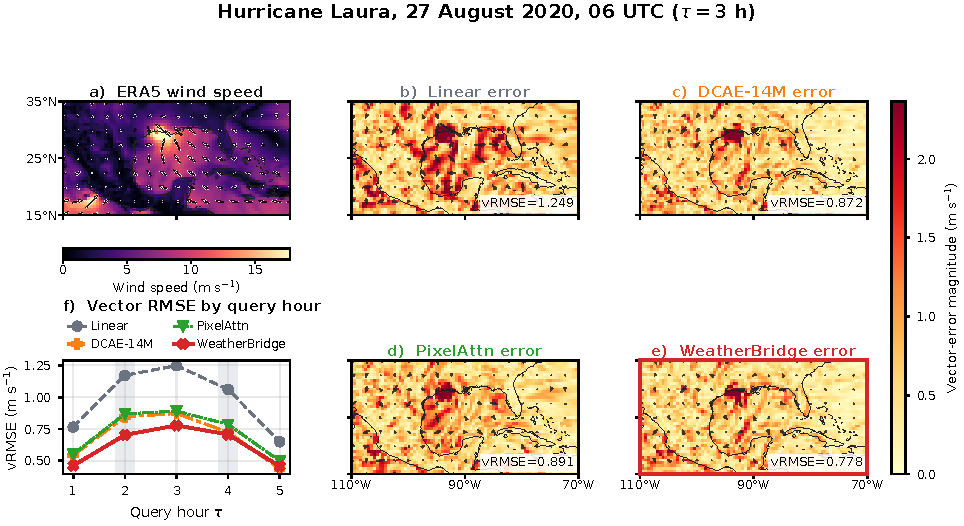
\includegraphics[width=0.94\linewidth,height=0.78\textheight,keepaspectratio]{images/fig_laura_wind10.pdf}
\captionof{figure}{10-m wind reconstruction during Hurricane Laura on 27 August 2020.
The left column shows ERA5 wind speed and direction at $\tau=3$ h and the
five-hour vector-RMSE trajectories. The right $2\times2$ block shows vector
error magnitude and direction for Linear Interp., WeatherDCAE-14M,
PixelAttn-VFI and WeatherBridge at the same query hour. Panel annotations give
cosine-latitude-weighted vector RMSE (vRMSE) over the fixed
$20{-}35^\circ$N, $80{-}105^\circ$W box. WeatherBridge has lower vRMSE than
both learned comparators at four of five interior hours; WeatherDCAE-14M is
lower at $\tau=5$ h.}
\label{fig:supp_laura_wind}
\end{supplementlandscape}

\FloatBarrier
\section{Twelve-hour per-channel errors}

Supplementary Figs.~\ref{fig:supp_channels_12h_body} and
\ref{fig:supp_channels_12h} resolve the twelve-hour interval-length ablation by
field. Model colours, markers and line styles match the six-hour comparison;
values should be compared within a field because the physical scales differ.

\begin{figure}[!htbp]
\centering

\includegraphics[width=\textwidth]{images/fig_channels_body_12h_phys.pdf}
\caption{Twelve-hour interval-length ablation for the 850-hPa and surface
fields in physical units. Shading marks hours excluded from training;
upward arrows mark clipped ModAFNO values beyond the displayed range.}
\label{fig:supp_channels_12h_body}
\end{figure}

\begin{figure}[!htbp]
\centering

\includegraphics[width=\textwidth]{images/fig_channels_app_12h_phys.pdf}
\caption{Twelve-hour interval-length ablation for the remaining pressure-level
fields in physical units. Shading marks hours excluded from training;
upward arrows mark clipped ModAFNO values beyond the displayed range.}
\label{fig:supp_channels_12h}
\end{figure}

\begin{table}[!htbp]
\centering
\caption{Matched-v2 12\,h interpolation on 2020 ERA5. Entries are mean $\pm$ standard deviation of the 24-channel macro RMSE across the indicated query hours. The standard deviation describes hour-to-hour variation, not sampling uncertainty over dates.}
\label{tab:main-12h}
\scriptsize
\setlength{\tabcolsep}{3.5pt}
\begin{tabular}{lrrrr}
\toprule
Model & Params (M) & Seen & Held out & All hours \\
\midrule
WeatherBridge & 14.3 & $\mathbf{0.099\pm0.033}$ & $\mathbf{0.133\pm0.008}$ & $\mathbf{0.108\pm0.032}$ \\
WeatherDCAE-14M & 14.4 & \underline{$0.107\pm0.034$} & \underline{$0.141\pm0.008$} & \underline{$0.117\pm0.033$} \\
PixelAttn-VFI & 14.7 & $0.122\pm0.038$ & $0.160\pm0.007$ & $0.133\pm0.037$ \\
SwinV2 & 7.9 & $0.168\pm0.058$ & $0.226\pm0.011$ & $0.184\pm0.056$ \\
S-DYff & 85.5 & $0.178\pm0.061$ & $0.240\pm0.012$ & $0.195\pm0.059$ \\
ModAFNO & 151.7 & $0.162\pm0.056$ & $0.369\pm0.018$ & $0.218\pm0.108$ \\
\midrule
\textit{Linear Interp.} & -- & $0.202\pm0.074$ & $0.278\pm0.015$ & $0.223\pm0.072$ \\
\bottomrule
\end{tabular}
\end{table}


Supplementary Fig.~\ref{fig:hres-best-fields} resolves four representative
same-trajectory results by forecast-lead bin; the aggregate and variable-group
scores are reported in Supplementary Table~\ref{tab:hres-same-trajectory} and
summarised in the main text.

\begin{table*}[!htbp]
\centering
\caption{Densifying a numerical forecast trajectory: both anchors and the target
are states of one IFS HRES run, separated by twelve hours, and the model
reconstructs the archived six-hour state between them. Sixteen 2021
initialisations, 39 windows each, 24 prognostic fields; scores are
latitude-weighted normalised RMSE and per-group columns give the reduction
relative to linear interpolation. All models are twelve-hour checkpoints
evaluated on the identical index. Internal architecture variants appear in the
separate ablation study.}
\label{tab:hres-same-trajectory}
\small
\setlength{\tabcolsep}{4pt}
\begin{tabular}{lcccccccc}
\toprule
Method & RMSE & vs.\ linear & T & U & V & Q & Z & surface \\
\midrule
Linear interpolation   & $0.2897$          & ---                & ---     & ---     & ---     & ---     & ---     & ---     \\
PixelAttn-VFI          & $0.2033$          & $+29.8\%$          & $+10.4$ & $+30.2$ & $+41.1$ & $+5.7$  & $-4.2$  & $+29.6$ \\
WeatherDCAE-14M        & $0.1765$          & $+39.1\%$          & $+20.1$ & $+39.3$ & $+49.4$ & $+13.5$ & $+15.5$ & $+38.3$ \\
\textbf{WeatherBridge} & $\mathbf{0.1664}$ & $\mathbf{+42.6\%}$ & $+25.1$ & $+42.5$ & $+50.0$ & $+32.2$ & $+20.7$ & $+40.4$ \\
\bottomrule
\end{tabular}
\end{table*}


\begin{figure*}[!htbp]
\centering
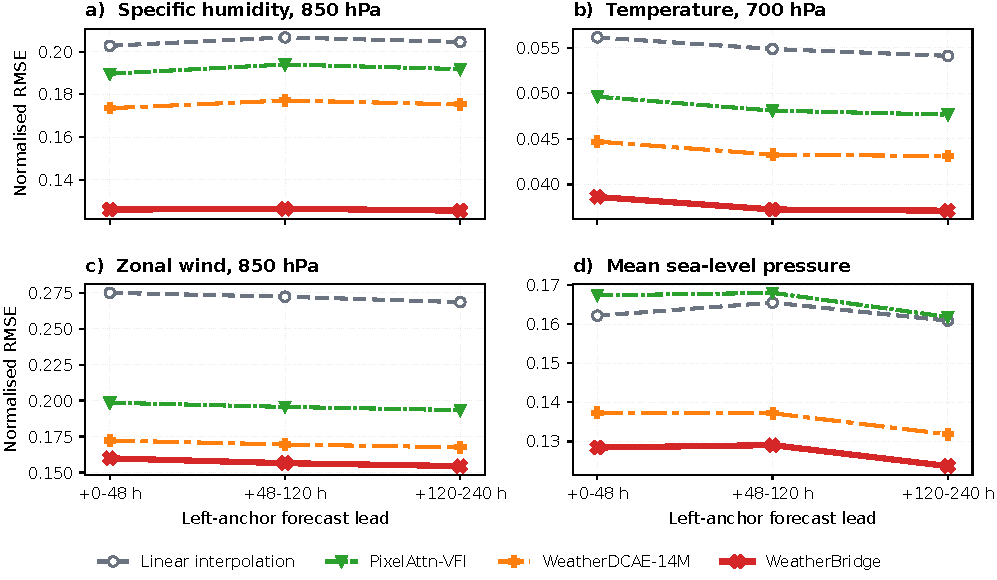
\includegraphics[width=0.94\textwidth]{images/fig_hres_best_fields.pdf}
\caption{Lead-resolved normalised RMSE for four representative fields in the
same-trajectory HRES experiment. The $x$ axis bins the forecast lead of the
left anchor; all curves use the same 16 initialisations and archived targets.
The panels were selected after evaluation as one field from each of four
physical families with a large WeatherBridge margin over the strongest plotted
competitor, so they are illustrative rather than a separate confirmatory test.
The main text retains the aggregate 24-field result.}
\label{fig:hres-best-fields}
\end{figure*}

\FloatBarrier
\section{Calendar-year transfer audit}

Supplementary Figs.~\ref{fig:supp_ood2021_body}--\ref{fig:supp_ood2021_levels}
use the same window construction, normalisation and query-hour split as the
2020 comparison. No learned model was trained on 2021, although these results
were inspected during development and are not a post-selection test.

% Auto-generated by tools/eval/export_2021_transfer_tex.py
\begin{table*}[!htbp]
\centering
\caption{Six-hour calendar transfer on the matched full-year 2021 index (7,295 window--hour samples). Seen hours are $\tau\in\{1,3,5\}$ and held-out hours are $\tau\in\{2,4\}$. Entries are mean $\pm$ standard deviation of 24-channel macro scores across the indicated query hours; this is descriptive hour-to-hour variation, not sampling uncertainty over dates. Lower RMSE and higher ACC are better. $\dagger$ marks legacy evaluator records that share the frozen index but predate corrected-grid and dataset-identity provenance. They are kept for context and do not meet the current provenance standard.}
\label{tab:transfer-2021}
\scriptsize
\setlength{\tabcolsep}{3pt}
\begin{tabular}{lrrrr}
\toprule
Model & Seen RMSE & Held-out RMSE & Avg. RMSE & ACC \\
\midrule
WeatherBridge & $\mathbf{0.055\pm0.019}$ & $\mathbf{0.074\pm0.003}$ & $\mathbf{0.062\pm0.017}$ & $\mathbf{0.995\pm0.002}$ \\
WeatherDCAE-14M & \underline{$0.063\pm0.021$} & \underline{$0.081\pm0.004$} & \underline{$0.070\pm0.018$} & \underline{$0.993\pm0.003$} \\
PixelAttn-VFI$^{\dagger}$ & $0.069\pm0.022$ & $0.091\pm0.003$ & $0.078\pm0.019$ & $0.992\pm0.004$ \\
SwinV2$^{\dagger}$ & $0.076\pm0.025$ & $0.095\pm0.003$ & $0.083\pm0.021$ & $0.992\pm0.004$ \\
S-DYff$^{\dagger}$ & $0.095\pm0.033$ & $0.119\pm0.001$ & $0.105\pm0.026$ & $0.990\pm0.005$ \\
ModAFNO$^{\dagger}$ & $0.096\pm0.035$ & $0.121\pm0.002$ & $0.106\pm0.028$ & $0.988\pm0.005$ \\
\midrule
Linear Interp. & $0.115\pm0.040$ & $0.144\pm0.001$ & $0.126\pm0.033$ & $0.986\pm0.007$ \\
\bottomrule
\end{tabular}
\end{table*}


\begin{figure*}[!ht]
\centering
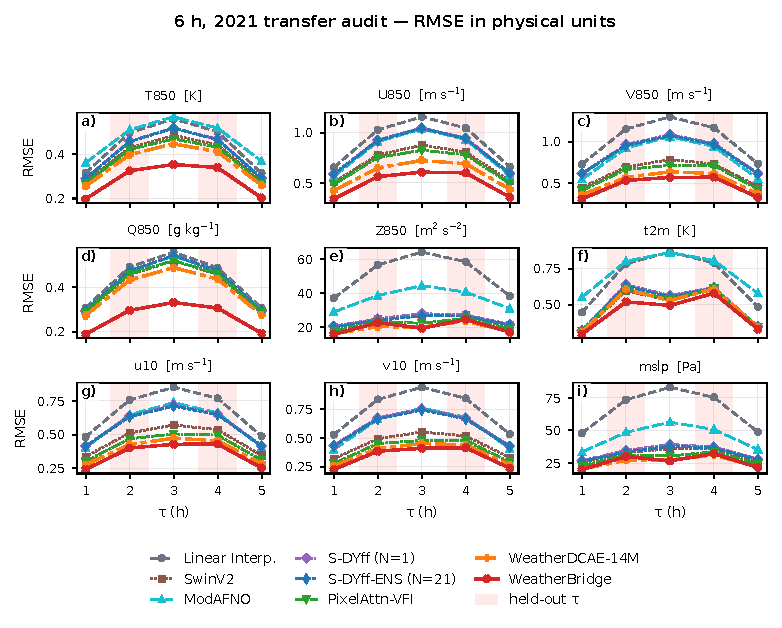
\includegraphics[width=\textwidth]{images/fig_channels_body_ood2021.pdf}
\caption{Six-hour per-channel RMSE in physical units in 2021 for representative
pressure-level and surface fields. Shading marks query hours excluded from
training. WeatherBridge is red.}
\label{fig:supp_ood2021_body}
\end{figure*}

\begin{figure*}[!ht]
\centering
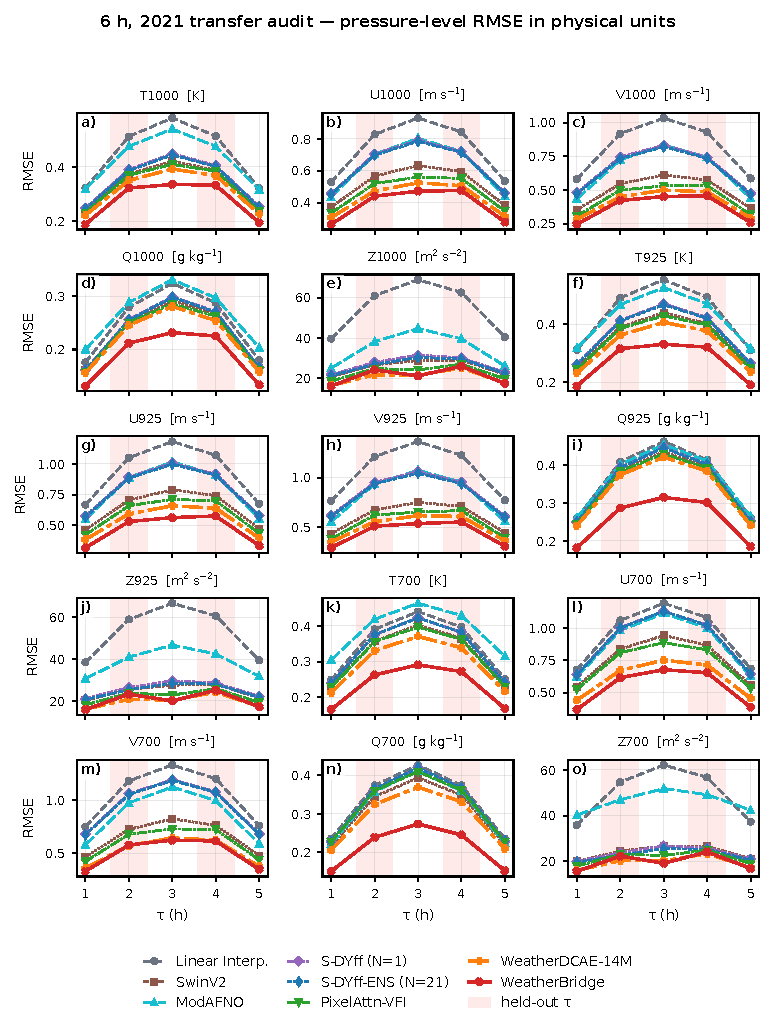
\includegraphics[width=\textwidth]{images/fig_channels_app_ood2021.pdf}
\caption{Six-hour RMSE in physical units in 2021 for the remaining pressure-level
channels. Shading marks query hours excluded from training.}
\label{fig:supp_ood2021_levels}
\end{figure*}

\FloatBarrier
\section{Full-query supervision control}
\label{sec:full-query-control}

The principal experiment withholds query hours 2 and 4 during optimisation.
Performance at those hours measures transfer. A counterpart trained on all
five interior hours estimates the benefit of direct supervision. Both
counterparts use the same 2014--2019 ERA5 pool, six-hour anchor construction,
24 fields and full-year 2020 and 2021 evaluation windows. Supplementary
Table~\ref{tab:full-query-protocol} records the checkpoint-level differences
that determine which comparisons support a causal interpretation.

For WeatherBridge, seed, optimiser-step budget, effective batch size,
precision and loss weights are matched; only the sampled query-hour set
changes. Full-query training reduces mean normalised RMSE at hours 2 and 4 by
8.77\% in 2020 and 8.78\% in 2021 (Supplementary
Fig.~\ref{fig:full-query-summary}). At the trained hours 1, 3 and 5, it changes
RMSE by $-0.35\%$ and $-0.34\%$, respectively. Thus the extra supervision
primarily improves the two hours omitted from sparse-query training.
The full-query WeatherBridge remains the best model in absolute
RMSE: 0.06015 in 2020 and 0.05991 in 2021 over all five hours, compared with
0.06466 and 0.06436 for WeatherDCAE-14M.

The WeatherBridge improvement at hours 2 and 4 is present in all 24 fields in
both years. The largest reductions occur for geopotential (18.0--18.8\%), MSLP
(17.3--17.5\%) and 2-m temperature (15.1--16.1\%); wind fields improve by
6.5--10.5\%, pressure-level temperature by 3.5--9.3\% and specific humidity by
2.8--7.6\%. The paired bootstrap defined in Methods gives a 95\%
interval of $[0.00650,0.00655]$ for sparse-minus-full nRMSE in 2020 and
$[0.00648,0.00653]$ in 2021. No draw is non-positive, so the corresponding
Monte Carlo tail probability is reported at its $1/5001$ resolution rather
than as zero.

The response depends on the architecture (Supplementary
Fig.~\ref{fig:full-query-field-hour}). SwinV2 gains about 2.1\% at hours 2 and
4, whereas S-DYff shows no gain. WeatherDCAE-14M and PixelAttn-VFI show
larger gains, but their full-query checkpoints receive 21,888 updates rather
than 13,136; those differences cannot be assigned to query-hour supervision
alone. WeatherBridge provides the matched comparison.
ModAFNO is omitted because its full-query run did not produce a complete
checkpoint. Linear interpolation has no training condition and therefore no
sparse-versus-full self-comparison.
The S-DYff comparison uses single stochastic reconstructions from each
checkpoint, with stochastic depth active at inference. It does not estimate
an ensemble-mean effect; the inference protocol and its difference from
original DYffusion are described in Methods.

\begin{table*}[!htbp]
\centering
\caption{Provenance of the six-hour sparse-query and full-query checkpoints.
The sparse-query runs draw $\tau\in\{1,3,5\}$; the full-query runs draw
$\tau\in\{1,2,3,4,5\}$. Both variants use the same 2014--2019 ERA5 pool and
are evaluated on identical 2020 and 2021 windows. Only the WeatherBridge pair
matches both optimiser budget and verified seed.}
\label{tab:full-query-protocol}
\footnotesize
\setlength{\tabcolsep}{4pt}
\begin{tabularx}{\textwidth}{
  >{\raggedright\arraybackslash}p{31mm}
  >{\centering\arraybackslash}p{29mm}
  >{\raggedright\arraybackslash}p{38mm}
  >{\raggedright\arraybackslash}X}
\toprule
\textbf{Architecture} & \textbf{Updates, sparse/full} &
\textbf{Seed evidence} & \textbf{Use in this control} \\
\midrule
WeatherBridge & 13,136 / 13,136 & Verified and matched &
Primary matched self-comparison \\
WeatherDCAE-14M & 13,136 / 21,888 & Same seed &
Diagnostic; extra optimisation confounds the query set \\
PixelAttn-VFI & 13,136 / 21,888 & Sparse seed not checkpoint-verified &
Diagnostic; update budget and seed evidence differ \\
SwinV2 & 17,520 / 17,520 & Sparse seed not checkpoint-verified &
Diagnostic despite matched update counts \\
S-DYff & 35,032 / 35,032 & Sparse seed not checkpoint-verified &
Diagnostic despite matched update counts \\
\bottomrule
\end{tabularx}
\end{table*}


\begin{figure*}[!htbp]
\centering
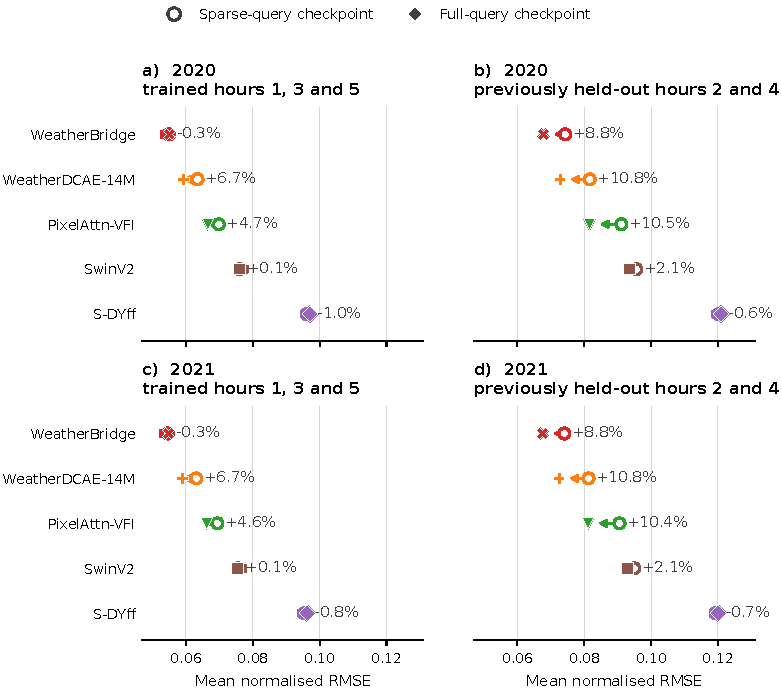
\includegraphics[width=0.98\textwidth]{images/fig_full_vs_heldout_summary.pdf}
\caption{Sparse-query versus full-query training on six-hour ERA5 intervals.
Open circles denote checkpoints trained at hours 1, 3 and 5; filled symbols
denote checkpoints trained at all five interior hours. Arrows point from the
sparse-query score to the full-query score, and labels give the relative RMSE
reduction. Lower normalised RMSE is better. Only WeatherBridge matches both
the verified seed and update budget. The other architectures show diagnostic
full-query sensitivity under the provenance constraints in Supplementary
Table~\ref{tab:full-query-protocol}.}
\label{fig:full-query-summary}
\end{figure*}

\begin{supplementlandscape}
\centering
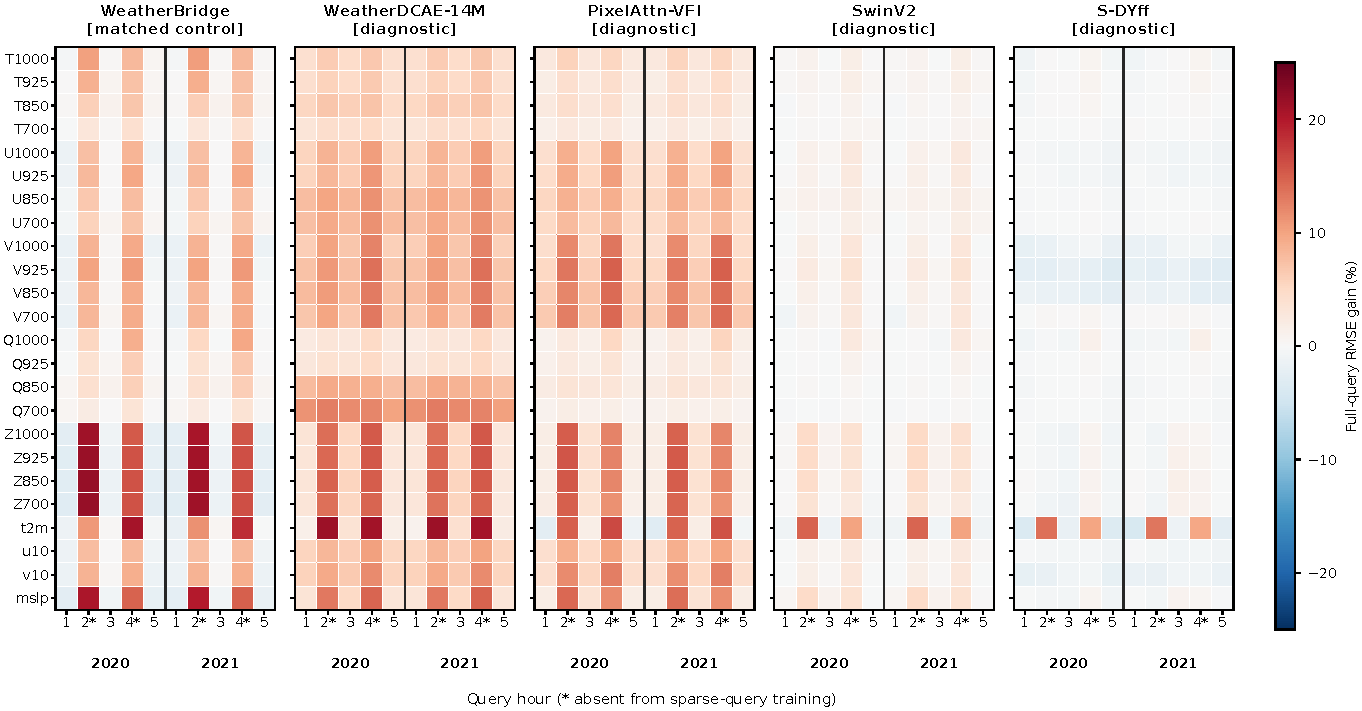
\includegraphics[width=0.96\linewidth,height=0.78\textheight,keepaspectratio]{images/fig_full_vs_heldout_field_hour.pdf}
\captionof{figure}{Field-by-hour change from sparse-query to full-query training.
Cells show $100(\mathrm{RMSE}_{\rm sparse}-\mathrm{RMSE}_{\rm full})/
\mathrm{RMSE}_{\rm sparse}$; red is an improvement and blue a regression.
Stars mark hours 2 and 4, which are absent from sparse-query training. Each
architecture contains the 2020 and 2021 results on the same colour scale.
WeatherBridge is the matched control; the remaining columns are diagnostic
because their seed or update-budget provenance is incomplete or unequal.}
\label{fig:full-query-field-hour}
\end{supplementlandscape}

\FloatBarrier
\section{Assimilation-window stratification}

The full-year six-hour comparison contains four anchor starts. Pairs beginning
at 00 and 12 UTC remain within one ERA5 4D-Var window, whereas those beginning
at 06 and 18 UTC cross the 09 or 21 UTC boundary. The ordering is unchanged in
all eight year--start strata, although WeatherBridge's advantage over
WeatherDCAE-14M is smaller for boundary-crossing pairs. This audit limits the
assimilation-window confound for RMSE. The spectral sample remains restricted
to 00/12 UTC, and the 2022 sample to 00 UTC.

% Auto-generated by tools/eval/summarize_utc_start_strata.py
\begin{table}[!ht]
\centering
\caption{Six-hour RMSE stratified by anchor start time. Starts at 00 and 12 UTC keep both anchors in one ERA5 4D-Var window; starts at 06 and 18 UTC cross the 09 or 21 UTC boundary. Scores are mean channel-wise normalised RMSE on the paired full-year index.}
\label{tab:utc-start-strata}
\small
\textbf{2020}\\[0.25em]
\begin{tabular}{lrrrr}
\toprule
Start UTC & WB & DCAE & Linear & WB vs DCAE \\
\midrule
00 (within) & 0.0608 & 0.0696 & 0.1274 & +12.6\% \\
06 (crosses 09 UTC) & 0.0680 & 0.0752 & 0.1328 & +9.5\% \\
12 (within) & 0.0616 & 0.0706 & 0.1290 & +12.7\% \\
18 (crosses 21 UTC) & 0.0672 & 0.0747 & 0.1314 & +10.0\% \\
Within-window pooled & 0.0612 & 0.0701 & 0.1282 & +12.7\% \\
Boundary-crossing pooled & 0.0676 & 0.0749 & 0.1321 & +9.7\% \\
\bottomrule
\end{tabular}
\par\vspace{0.6em}
\textbf{2021}\\[0.25em]
\begin{tabular}{lrrrr}
\toprule
Start UTC & WB & DCAE & Linear & WB vs DCAE \\
\midrule
00 (within) & 0.0605 & 0.0693 & 0.1269 & +12.6\% \\
06 (crosses 09 UTC) & 0.0678 & 0.0748 & 0.1323 & +9.4\% \\
12 (within) & 0.0613 & 0.0702 & 0.1283 & +12.6\% \\
18 (crosses 21 UTC) & 0.0670 & 0.0744 & 0.1310 & +9.9\% \\
Within-window pooled & 0.0609 & 0.0697 & 0.1276 & +12.6\% \\
Boundary-crossing pooled & 0.0674 & 0.0746 & 0.1317 & +9.6\% \\
\bottomrule
\end{tabular}
\end{table}


\FloatBarrier
\section{Conservative robustness sensitivity}

The internal sensitivity defined in Methods checks fieldwise regressions
against WeatherDCAE-14M alongside aggregate accuracy, parameter count,
latency and HRES transfer. It was defined during development; it is
reported separately from the primary held-out query-hour comparison.

This rule retains WeatherDCAE-14M because WeatherBridge has local regressions
despite lower aggregate and held-out RMSE. Supplementary
Table~\ref{tab:selector-diagnostics} gives the temporal-curvature
outcomes. Supplementary Table~\ref{tab:vector-sht} gives representative
vector-SHT values; Supplementary Data~1 contains the complete families.

% Source SHA-256: 855a37521762fda33a382e77f14a35cc30ea01f9a0ee200061b1b7b546ee4652
\begin{table}[!ht]
\centering
\caption{Selector diagnostics for WeatherBridge against WeatherDCAE-14M. Lower is better. Curvature intervals use paired seven-day blocks ($n=53$). In the physical diagnostics (Supplementary Data~1), lower-tropospheric moisture bias is the sole Holm-significant regression in every row.}
\label{tab:selector-diagnostics}
\small
\setlength{\tabcolsep}{3pt}
\begin{tabular}{@{}lccc@{}}
\toprule
Interval, year & \shortstack{WeatherBridge\\curvature} & \shortstack{WeatherDCAE\\curvature} & $\Delta$ [95\% CI] \\
\midrule
6\,h, 2020 & 0.08570 & 0.08477 & +0.00094 [+0.00076, +0.00111] \\
6\,h, 2021 & 0.08533 & 0.08427 & +0.00106 [+0.00090, +0.00122] \\
12\,h, 2020 & 0.09048 & 0.08784 & +0.00264 [+0.00257, +0.00271] \\
12\,h, 2021 & 0.08980 & 0.08719 & +0.00262 [+0.00254, +0.00268] \\
\bottomrule
\end{tabular}
\end{table}


% Source SHA-256: 855a37521762fda33a382e77f14a35cc30ea01f9a0ee200061b1b7b546ee4652
\begin{table}[!ht]
\centering
\caption{Vector-SHT signed cospectrum for 850-hPa wind in 2020. One is ideal; higher is better. Query hours include one held-out and one trained time per interval. Intervals are paired over calendar-week blocks. Supplementary Data~1 contains the complete multiplicity-corrected vector family.}
\label{tab:vector-sht}
\small
\begin{tabular}{@{}rrlccc@{}}
\toprule
Interval & $\tau$ & Component & WeatherBridge & WeatherDCAE & $\Delta$ [95\% CI] \\
\midrule
6\,h & 2 & Spheroidal & 0.973 & 0.966 & +0.007 [+0.006, +0.007] \\
6\,h & 2 & Toroidal & 0.881 & 0.853 & +0.027 [+0.027, +0.028] \\
6\,h & 3 & Spheroidal & 0.969 & 0.958 & +0.011 [+0.010, +0.011] \\
6\,h & 3 & Toroidal & 0.862 & 0.821 & +0.041 [+0.041, +0.042] \\
12\,h & 5 & Spheroidal & 0.852 & 0.828 & +0.024 [+0.023, +0.025] \\
12\,h & 5 & Toroidal & 0.546 & 0.523 & +0.022 [+0.021, +0.024] \\
12\,h & 8 & Spheroidal & 0.860 & 0.833 & +0.027 [+0.026, +0.028] \\
12\,h & 8 & Toroidal & 0.588 & 0.561 & +0.027 [+0.026, +0.028] \\
\bottomrule
\end{tabular}
\end{table}


\FloatBarrier
\section{Architecture ablation study}

% Auto-generated by tools/eval/export_architecture_ablation_tex.py
\begin{table}[!ht]
\centering
\caption{Transport-architecture ablation. RMSE is the 24-field full-year mean; lower is better. Internal variants are confined to this audit table; the main comparison uses WeatherBridge.}
\label{tab:architecture-ablation}
\footnotesize
\setlength{\tabcolsep}{3.5pt}
\begin{tabularx}{\textwidth}{@{}l>{\raggedright\arraybackslash}Xrrrr@{}}
\toprule
Variant & Architectural difference & \shortstack{Params\\(M)} & \shortstack{6\,h\\2020} & \shortstack{6\,h\\2021} & \shortstack{12\,h\\2020} \\
\midrule
WeatherBridge & Transport trunk + spectral supervision & 14.3 & 0.0626 & 0.0624 & 0.1081 \\
Detail & + transported anchor-detail bypass & 14.3 & 0.0625 & 0.0622 & 0.1090 \\
Refine & Latent transformer; shared heads; no mass head & 13.7 & 0.0624 & 0.0622 & 0.1096 \\
\bottomrule
\end{tabularx}
\end{table}


The retrained Refine variant, defined in Methods, lowered aggregate six-hour
ERA5 RMSE, but two field--hour regressions remained in the inspected 2021
transfer year: temperature (T2m) regressions at $\tau=1$ and $\tau=5$, with
one-sided Holm-adjusted $p=0.024$ each. It also lost all three paired IFS HRES
seeds, and the conservative robustness sensitivity rejects it.
Supplementary Data~1 retains its configuration, checkpoints and paired
statistics.

The same sensitivity also rejects Detail, the anchor-detail bypass variant
defined in Methods.

Refine and Detail lower six-hour full-year ERA5 RMSE by less than one per cent
relative to WeatherBridge, but transfer less reliably across data sources.
Refine loses all three paired IFS HRES seeds at both horizons; Detail loses its
only completed seed pair at both horizons, leaving its cross-source evidence
incomplete. WeatherBridge has the lowest twelve-hour ERA5 RMSE of the three and
wins all three twelve-hour HRES seed pairs. We retain it as the representative
transport formulation. The stricter multi-metric rule retains
WeatherDCAE-14M as the conservative reference.

The retrained branches above change several mechanisms at once. To isolate
components used by the retained checkpoint, we also apply
same-checkpoint inference lesions. Disabling the acceleration term increases
aggregate RMSE by 2.16\%, while forcing the warped-anchor gate to zero
increases it by 60.54\%. Disabling the hydrostatic head increases aggregate
RMSE by only 0.04\%, as it changes five of 24 channels, but all 25 affected
geopotential/MSLP field--hour cells worsen after Holm correction. Averaged
over the five query hours, hydrostatic-balance MSE increases by 1.06\%
(Supplementary Table~\ref{tab:component-lesions}, panel b). The transport-off arm
retains the learned residual corrections and isolates warped-anchor transport
without reducing the model to linear interpolation. No arm is retrained.

% Auto-generated by tools/eval/export_component_lesions_tex.py
\begin{table}[!ht]
\centering
\caption{Same-checkpoint inference lesions on the full-year 2020 six-hour index. No arm is retrained. Positive $\Delta$ and percentage values denote degradation relative to intact WeatherBridge. All three aggregate lesion tests reach the Monte Carlo resolution limit ($1/5001$) under paired seven-day-block permutation. Panel b resolves the hydrostatic lesion over geopotential $Z$ at four pressure levels and mean sea-level pressure (MSLP); RMSE and percentage change are computed from averages across the five query hours, followed by the minimum--maximum hourly change in brackets.}
\label{tab:component-lesions}
\small
\setlength{\tabcolsep}{4pt}
\begin{tabularx}{\textwidth}{@{}>{\raggedright\arraybackslash}Xrrr@{}}
\multicolumn{4}{@{}l}{\textbf{a. Aggregate lesions}} \\
\toprule
Inference arm & RMSE & $\Delta$ vs intact & Change (\%) \\
\midrule
Intact WeatherBridge & 0.06263 & +0.00000 & +0.00 \\
Acceleration disabled & 0.06398 & +0.00135 & +2.16 \\
Warped-anchor transport disabled & 0.10055 & +0.03792 & +60.54 \\
Hydrostatic head disabled & 0.06265 & +0.00003 & +0.04 \\
\bottomrule
\end{tabularx}
\medskip
\begin{tabularx}{\textwidth}{@{}>{\raggedright\arraybackslash}Xrrr@{}}
\multicolumn{4}{@{}l}{\textbf{b. Hydrostatic-head target fields}} \\
\toprule
Field & Intact RMSE & Head-off RMSE & Change (\%) \\
\midrule
$Z_{1000}$ & 0.02326 & 0.02342 & +0.69 [+0.24, +1.06] \\
$Z_{925}$ & 0.01846 & 0.01857 & +0.59 [+0.21, +0.87] \\
$Z_{850}$ & 0.01441 & 0.01450 & +0.66 [+0.27, +0.97] \\
$Z_{700}$ & 0.00938 & 0.00945 & +0.77 [+0.25, +1.15] \\
MSLP & 0.02360 & 0.02378 & +0.74 [+0.31, +1.13] \\
\bottomrule
\end{tabularx}
\end{table}


\FloatBarrier
\section{Anchor-order diagnostic}

Neither principal architecture is equivariant to exchanging the two anchors.
For WeatherBridge, the exchange RMSE is 0.287 in 2020 and 0.285 in 2021,
respectively 3.49 and 3.44 times its forward reconstruction error. The
corresponding WeatherDCAE-14M ratios are 3.01 and 2.98. ``Bidirectional''
refers to the two predicted transport directions. The complete interpolation
map is not reversible because the input stack and learned path assign distinct
roles to the left and right anchors.

% Auto-generated by tools/eval/export_anchor_exchange_tex.py
\begin{table}[!ht]
\centering
\caption{Anchor-exchange diagnostic on the six-hour task. Exchange RMSE compares $f(x_0,x_T,t)$ with $f(x_T,x_0,1-t)$; forward RMSE compares the first prediction with ERA5. Lower is better. The 48-endpoint, 240-window sample per year is diagnostic and was not used for selection.}
\label{tab:anchor-exchange}
\begin{tabular}{llrrr}
\toprule
Model & Year & Exchange RMSE & Forward RMSE & Ratio \\
\midrule
WeatherBridge & 2020 & 0.287 & 0.082 & 3.49 \\
WeatherBridge & 2021 & 0.285 & 0.083 & 3.44 \\
WeatherDCAE-14M & 2020 & 0.278 & 0.092 & 3.01 \\
WeatherDCAE-14M & 2021 & 0.276 & 0.093 & 2.98 \\
\bottomrule
\end{tabular}
\end{table}


\FloatBarrier
\section{Twelve-hour spectral amplitude}

Supplementary Fig.~\ref{fig:supp_spectra_12h} shows spectral amplitude. The
scalar and vector-SHT tables below report the signed cospectrum and vector-field
tests needed to assess coefficient alignment.

\begin{figure}[!htbp]
\centering

\includegraphics[width=\textwidth]{images/fig_spectra_ratio_hard.pdf}
\caption{Twelve-hour spectral power retention. Rows show Q850 and V850; columns
compare a trained query hour ($\tau=5$) with a held-out hour ($\tau=6$). Curves
show the model-to-ERA5 power ratio over $\ell\in[80,180]$; one is ideal.
WeatherBridge has the lowest mean absolute log-ratio error for Q850 in both
columns and is shown in solid red.}
\label{fig:supp_spectra_12h}
\end{figure}

% Auto-generated by tools/eval/build_sh_per_channel_table_12h.py
% Source: metrics/journal_spectra_v6/6h_2020/*.npz  (7 displayed models × 24 channels)
\begin{table*}[!htbp]
\centering
\caption{Per-channel spherical-harmonic high-frequency preservation ratio $R_{\mathrm{HF}} = \sum_{\ell \geq 80} E_{\mathrm{pred}}(\ell) / \sum_{\ell \geq 80} E_{\mathrm{GT}}(\ell)$ for the 6\,h leaderboard, averaged over $\tau \in \{1, 2, 3, 4, 5\}$ across all 24 prognostic channels (5 PL variables $\times$ 4 levels = 20 + 4 surface). $R_{\mathrm{HF}} = 1$ = perfect spectral fidelity; values $<1$ indicate HF energy under-prediction. Per-row \textbf{best} (closest to 1.0) and \underline{worst} (farthest from 1.0) highlighted. Block means aggregate over the 4 PL levels per variable; the surface block mean uses the 4 surface fields.}
\label{tab:sh_per_channel_6h}
\small
\setlength{\tabcolsep}{4pt}
\resizebox{\textwidth}{!}{%
\begin{tabular}{lrrrrrrr}
\toprule
Channel & WeatherBridge & WeatherDCAE-14M & PixelAttn-VFI & SwinV2 & ModAFNO & S-DYff & Linear Interp. \\
\midrule
T1000 & \textbf{0.884} & 0.879 & 0.877 & 0.871 & 0.874 & 0.878 & \underline{0.851} \\
T925 & \textbf{0.857} & 0.843 & 0.826 & 0.825 & 0.818 & 0.823 & \underline{0.796} \\
T850 & \textbf{0.811} & 0.791 & 0.768 & 0.776 & 0.773 & 0.777 & \underline{0.751} \\
T700 & 0.771 & \textbf{0.773} & 0.765 & 0.765 & 0.772 & 0.768 & \underline{0.753} \\
\textit{mean(T*)} & 0.831 & 0.821 & 0.809 & 0.809 & 0.809 & 0.812 & 0.788 \\
\midrule
U1000 & \textbf{0.900} & 0.893 & 0.855 & 0.841 & 0.804 & 0.818 & \underline{0.771} \\
U925 & \textbf{0.889} & 0.889 & 0.851 & 0.836 & 0.792 & 0.801 & \underline{0.756} \\
U850 & \textbf{0.872} & 0.867 & 0.804 & 0.806 & 0.772 & 0.780 & \underline{0.742} \\
U700 & \textbf{0.823} & 0.821 & 0.729 & 0.753 & 0.727 & 0.735 & \underline{0.704} \\
\textit{mean(U*)} & 0.871 & 0.867 & 0.810 & 0.809 & 0.774 & 0.784 & 0.743 \\
\midrule
V1000 & \textbf{0.911} & 0.899 & 0.863 & 0.842 & 0.781 & 0.809 & \underline{0.749} \\
V925 & \textbf{0.902} & 0.890 & 0.849 & 0.830 & 0.752 & 0.783 & \underline{0.730} \\
V850 & \textbf{0.891} & 0.885 & 0.817 & 0.817 & 0.757 & 0.761 & \underline{0.718} \\
V700 & \textbf{0.852} & 0.846 & 0.760 & 0.757 & 0.708 & 0.709 & \underline{0.672} \\
\textit{mean(V*)} & 0.889 & 0.880 & 0.822 & 0.812 & 0.750 & 0.766 & 0.717 \\
\midrule
Q1000 & 0.854 & 0.851 & \textbf{0.857} & 0.847 & 0.854 & 0.857 & \underline{0.837} \\
Q925 & \textbf{0.798} & 0.762 & 0.759 & 0.751 & 0.755 & 0.762 & \underline{0.738} \\
Q850 & \textbf{0.827} & 0.762 & 0.743 & 0.736 & 0.740 & 0.754 & \underline{0.715} \\
Q700 & \textbf{0.764} & 0.743 & 0.731 & 0.736 & 0.740 & 0.752 & \underline{0.716} \\
\textit{mean(Q*)} & 0.811 & 0.780 & 0.773 & 0.768 & 0.772 & 0.781 & 0.751 \\
\midrule
Z1000 & 0.928 & \textbf{0.938} & 0.920 & 0.930 & 0.924 & 0.935 & \underline{0.901} \\
Z925 & 0.918 & \textbf{0.928} & 0.913 & 0.921 & 0.914 & 0.922 & \underline{0.884} \\
Z850 & 0.899 & \textbf{0.911} & 0.895 & 0.903 & 0.893 & 0.898 & \underline{0.857} \\
Z700 & 0.844 & \textbf{0.868} & 0.831 & 0.857 & 0.865 & 0.826 & \underline{0.759} \\
\textit{mean(Z*)} & 0.897 & 0.911 & 0.890 & 0.903 & 0.899 & 0.895 & 0.850 \\
\midrule
t2m & 0.926 & 0.932 & 0.948 & 0.932 & 0.938 & \textbf{0.953} & \underline{0.920} \\
u10 & \textbf{0.902} & 0.896 & 0.858 & 0.841 & 0.803 & 0.818 & \underline{0.771} \\
v10 & \textbf{0.911} & 0.901 & 0.865 & 0.842 & 0.777 & 0.807 & \underline{0.746} \\
mslp & 0.925 & \textbf{0.934} & 0.917 & 0.925 & 0.921 & 0.931 & \underline{0.899} \\
\textit{mean(surface)} & 0.916 & 0.916 & 0.897 & 0.885 & 0.860 & 0.877 & 0.834 \\
\midrule
\textbf{mean (24ch)} & 0.869 & 0.863 & 0.833 & 0.831 & 0.811 & 0.819 & 0.781 \\
\bottomrule
\end{tabular}
}
\end{table*}


% Auto-generated by tools/eval/build_sh_per_channel_table_12h.py
% Source: metrics/journal_spectra_v6/12h_2020/*.npz  (7 displayed models × 24 channels)
\begin{table*}[!htbp]
\centering
\caption{Per-channel spherical-harmonic high-frequency preservation ratio $R_{\mathrm{HF}} = \sum_{\ell \geq 80} E_{\mathrm{pred}}(\ell) / \sum_{\ell \geq 80} E_{\mathrm{GT}}(\ell)$ for the 12\,h leaderboard, averaged over $\tau \in \{1, 2, 3, 4, 5, 6, 7, 8, 9, 10, 11\}$ across all 24 prognostic channels (5 PL variables $\times$ 4 levels = 20 + 4 surface). $R_{\mathrm{HF}} = 1$ = perfect spectral fidelity; values $<1$ indicate HF energy under-prediction. Per-row \textbf{best} (closest to 1.0) and \underline{worst} (farthest from 1.0) highlighted. Block means aggregate over the 4 PL levels per variable; the surface block mean uses the 4 surface fields.}
\label{tab:sh_per_channel_12h}
\small
\setlength{\tabcolsep}{4pt}
\resizebox{\textwidth}{!}{%
\begin{tabular}{lrrrrrrr}
\toprule
Channel & WeatherBridge & WeatherDCAE-14M & PixelAttn-VFI & SwinV2 & ModAFNO & S-DYff & Linear Interp. \\
\midrule
T1000 & 0.794 & \textbf{0.818} & \underline{0.792} & 0.804 & 0.802 & 0.810 & 0.802 \\
T925 & 0.771 & \textbf{0.781} & \underline{0.743} & 0.754 & 0.755 & 0.762 & 0.752 \\
T850 & 0.731 & \textbf{0.743} & \underline{0.704} & 0.726 & 0.733 & 0.732 & 0.723 \\
T700 & \underline{0.712} & \textbf{0.753} & 0.744 & 0.737 & 0.740 & 0.744 & 0.733 \\
\textit{mean(T*)} & 0.752 & 0.774 & 0.746 & 0.755 & 0.757 & 0.762 & 0.752 \\
\midrule
U1000 & 0.753 & \textbf{0.795} & 0.710 & 0.721 & \underline{0.700} & 0.731 & 0.728 \\
U925 & 0.773 & \textbf{0.812} & 0.734 & 0.708 & \underline{0.691} & 0.721 & 0.715 \\
U850 & 0.744 & \textbf{0.775} & \underline{0.650} & 0.703 & 0.684 & 0.704 & 0.703 \\
U700 & 0.667 & \textbf{0.694} & \underline{0.546} & 0.681 & 0.658 & 0.681 & 0.679 \\
\textit{mean(U*)} & 0.735 & 0.769 & 0.660 & 0.703 & 0.683 & 0.709 & 0.706 \\
\midrule
V1000 & 0.775 & \textbf{0.794} & 0.720 & 0.693 & \underline{0.666} & 0.716 & 0.718 \\
V925 & 0.790 & \textbf{0.811} & 0.718 & 0.675 & \underline{0.642} & 0.692 & 0.709 \\
V850 & 0.742 & \textbf{0.750} & \underline{0.625} & 0.678 & 0.630 & 0.664 & 0.695 \\
V700 & 0.649 & 0.652 & \underline{0.506} & 0.644 & 0.579 & \textbf{0.679} & 0.669 \\
\textit{mean(V*)} & 0.739 & 0.752 & 0.642 & 0.672 & 0.629 & 0.688 & 0.698 \\
\midrule
Q1000 & \underline{0.767} & \textbf{0.798} & 0.777 & 0.780 & 0.777 & 0.785 & 0.780 \\
Q925 & \textbf{0.719} & 0.714 & \underline{0.672} & 0.698 & 0.675 & 0.702 & 0.699 \\
Q850 & \textbf{0.721} & 0.695 & \underline{0.631} & 0.664 & 0.663 & 0.673 & 0.665 \\
Q700 & \textbf{0.673} & 0.668 & \underline{0.641} & 0.662 & 0.660 & 0.668 & 0.661 \\
\textit{mean(Q*)} & 0.720 & 0.719 & 0.680 & 0.701 & 0.694 & 0.707 & 0.701 \\
\midrule
Z1000 & \underline{0.874} & 0.909 & 0.875 & 0.898 & 0.903 & \textbf{0.933} & 0.890 \\
Z925 & \underline{0.872} & 0.909 & 0.875 & 0.892 & 0.908 & \textbf{0.928} & 0.879 \\
Z850 & 0.856 & 0.899 & 0.860 & 0.873 & \textbf{0.935} & 0.914 & \underline{0.847} \\
Z700 & 0.801 & 0.871 & 0.829 & 0.813 & 1.242 & \textbf{0.888} & \underline{0.732} \\
\textit{mean(Z*)} & 0.851 & 0.897 & 0.860 & 0.869 & 0.997 & 0.916 & 0.837 \\
\midrule
t2m & \underline{0.846} & 0.896 & 0.882 & 0.893 & 0.893 & \textbf{0.899} & 0.890 \\
u10 & 0.755 & \textbf{0.800} & 0.711 & 0.719 & \underline{0.697} & 0.729 & 0.727 \\
v10 & 0.777 & \textbf{0.797} & 0.721 & 0.689 & \underline{0.658} & 0.711 & 0.714 \\
mslp & 0.870 & 0.902 & \underline{0.869} & 0.891 & 0.902 & \textbf{0.924} & 0.884 \\
\textit{mean(surface)} & 0.812 & 0.849 & 0.796 & 0.798 & 0.787 & 0.816 & 0.804 \\
\midrule
\textbf{mean (24ch)} & 0.768 & 0.793 & 0.731 & 0.750 & 0.758 & 0.766 & 0.750 \\
\bottomrule
\end{tabular}
}
\end{table*}


\FloatBarrier
\section{Diagnostic physical and regional summaries}

The balance ratios use 180 uniformly spaced windows, while the diurnal errors
aggregate four regions, 12 months and three surface fields. These reduced-sample
diagnostics are descriptive; the full-year physical suite supplies the paired
robustness analysis.

\begin{table}[!htbp]
\centering
\caption{Diagnostic-balance ratios relative to ERA5 over 180 uniformly spaced 2020 anchor windows and all interior hours. One is the reference value; bold marks the closest ratio within each horizon and diagnostic.}
\label{tab:physics_balance}
\small
\setlength{\tabcolsep}{4pt}
\begin{tabular}{llrrr}
\toprule
Horizon & Model & Ageo 850 & Ageo 700 & Hydrostatic \\
\midrule
6\,h & WeatherBridge & 0.949 & 0.940 & 0.992 \\
 & WeatherDCAE-14M & \textbf{0.962} & \textbf{0.962} & \textbf{0.994} \\
 & Linear Interp. & 0.936 & 0.903 & 0.993 \\
\midrule
12\,h & WeatherBridge & 0.924 & 0.920 & 0.985 \\
 & WeatherDCAE-14M & \textbf{0.958} & \textbf{0.981} & \textbf{0.992} \\
 & Linear Interp. & 0.926 & 0.878 & \textbf{0.992} \\
\bottomrule
\end{tabular}
\end{table}


\begin{table}[!htbp]
\centering
\caption{Regional diurnal-cycle errors over four regions, 12 months and three surface fields (144 strata). Amplitude error is $|A_{\mathrm{recon}}/A_{\mathrm{ERA5}}-1|$; peak error is the circular local-time difference. Lower is better; bold marks the lowest value per horizon.}
\label{tab:diurnal}
\small
\setlength{\tabcolsep}{5pt}
\begin{tabular}{llrr}
\toprule
Horizon & Model & Amplitude error & Peak error (h) \\
\midrule
6\,h & WeatherBridge & \textbf{0.043} & \textbf{0.507} \\
 & WeatherDCAE-14M & 0.047 & 0.674 \\
 & Linear Interp. & 0.170 & 1.569 \\
\midrule
12\,h & WeatherBridge & \textbf{0.068} & \textbf{0.562} \\
 & WeatherDCAE-14M & 0.070 & 0.660 \\
 & Linear Interp. & 0.508 & 3.597 \\
\bottomrule
\end{tabular}
\end{table}


\FloatBarrier
\section{Training and architecture inventory}

Tables~\ref{tab:protocol_summary} and \ref{tab:hyperparams} record
the training budgets and architecture settings of the reported checkpoints.

\begin{table*}[!htbp]
\centering
\caption{Training protocol for the reported checkpoints. Models grouped
within a row share the training years, epoch budget and optimiser-step
count. Every run uses the same 24 fields and peak learning rate $10^{-4}$.}
\label{tab:protocol_summary}
\footnotesize
\setlength{\tabcolsep}{4pt}
\begin{tabularx}{\textwidth}{
  >{\raggedright\arraybackslash}X
  >{\centering\arraybackslash}p{20mm}
  >{\centering\arraybackslash}p{25mm}
  >{\centering\arraybackslash}p{28mm}}
\toprule
\textbf{Setting} & \textbf{Years} & \textbf{Epochs} & \textbf{Updates} \\
\midrule
WeatherBridge, WeatherDCAE-14M,
PixelAttn-VFI (6\,h) & 2014--2019 & 8 & 13,136 \\
SwinV2 (6\,h) & 2014--2019 & 8 & 17,520 \\
ModAFNO, S-DYff (6\,h) & 2014--2019 & 8 & 35,032 \\
WeatherBridge, WeatherDCAE-14M,
PixelAttn-VFI (12\,h) & 2017--2019 & 10 & 10,930 \\
SwinV2, S-DYff (12\,h) & 2017--2019 & 10 & 5,470 \\
ModAFNO (12\,h) & 2017--2019 & 10 & 21,870 \\
\bottomrule
\end{tabularx}
\end{table*}


\begin{table*}[!htbp]
\centering
\caption{Per-variant architecture settings. Parameter counts come from the
reported checkpoint state dictionaries; \emph{n-modes} gives the
spherical-FNO truncation (latitude$\times$longitude).}
\label{tab:hyperparams}
\small
\setlength{\tabcolsep}{4pt}
\begin{tabular}{p{0.22\textwidth}r p{0.62\textwidth}}
\toprule
\textbf{Variant} & \textbf{Params} & \textbf{Hyperparameters} \\
\midrule
WeatherBridge & 14.3\,M & hidden 72; three-level circular-padded U-Net; second-order transport, blend, pyramid residual, SFNO and mass-field heads; replicated-latitude high-pass boundary; FFT-magnitude term on the advected-channel mask \\
WeatherDCAE-14M & 14.4\,M & block-out 64/128/256, layers 3/3/3, latent 256; longitude-periodic, scalar-style pole-reflected convolutions \\
\midrule
SwinV2 & 7.9\,M & embed 256, depth 8, heads 8, window $5{\times}9$, patch 4 \\
ModAFNO (6\,h) & 36.9\,M & embed 256, depth 8, blocks 8, MLP ratio 2 \\
ModAFNO (12\,h) & 151.7\,M & embed 512, depth 12, blocks 8, MLP ratio 2 \\
S-DYff (6\,h) & 101.3\,M & embed 128, depth 4, n-modes $16{\times}32$, $K{=}5$ refine \\
S-DYff (12\,h) & 85.5\,M & embed 96, depth 6, n-modes $16{\times}32$, $K{=}5$ refine \\
PixelAttn-VFI & 14.7\,M & hidden 72; three levels; shared anchor encoder; bottleneck self-attention and AdaLN-Zero; mean-endpoint decoder skips \\
\bottomrule
\end{tabular}
\end{table*}


\FloatBarrier
\section{Forecast-anchor spectral audit}

The four-cell audit below accompanies the adapted IFS HRES result in the main
text. It separates small-scale amplitude from coefficient alignment: improved
coherence and signed cospectrum do not imply uniformly improved spectral
energy or shape.

\begin{table*}[!htbp]
\caption{Independent 2022 forecast-anchor spectral differences over
$\ell=80$--$180$. Values are the frozen coefficient adapter minus Linear Interp.;
negative is better for energy and shape error, whereas positive is better for
coherence and signed cospectrum. $\dagger$ denotes Holm-adjusted $p<0.05$
over the two fields within each metric and query hour.}
\label{tab:supp_nwp_spectra_2022}
\centering
\small
\setlength{\tabcolsep}{4pt}
\begin{tabular}{clrrrr}
\toprule
$\tau$ & Field & $\Delta$ energy error $\downarrow$ &
$\Delta$ shape error $\downarrow$ & $\Delta$ coherence $\uparrow$ &
$\Delta$ signed cospectrum $\uparrow$ \\
\midrule
2 & Q850 & $+0.0009\dagger$ & $+0.0023\dagger$ & $+0.0064\dagger$ & $+0.0069\dagger$ \\
2 & U850 & $+0.0044\dagger$ & $-0.0008\dagger$ & $+0.0045\dagger$ & $+0.0041\dagger$ \\
3 & Q850 & $-0.0006$ & $+0.0093\dagger$ & $+0.0112\dagger$ & $+0.0122\dagger$ \\
3 & U850 & $+0.0091\dagger$ & $-0.0001$ & $+0.0108\dagger$ & $+0.0099\dagger$ \\
\bottomrule
\end{tabular}
\end{table*}


\FloatBarrier
\section{Coefficient adapter by field}

Supplementary Fig.~\ref{fig:nwp_adapter_2022} uses 16 IFS HRES
initialisations chosen before the 2022 evaluation. Pairs of states separated by
six hours are drawn from the same forecast trajectory and used as the two
anchors. Linear interpolation, WeatherDCAE-14M, WeatherBridge and its frozen
coefficient adapter reconstruct the five intervening hourly states; each
prediction is compared with ERA5 at the same valid time. Here, $\tau$ denotes
the offset within an HRES anchor pair rather than forecast lead time. These
scores include both interpolation error and the mismatch between HRES and
ERA5, so they are not conventional HRES forecast-skill curves.

\begin{figure}[!ht]
\centering
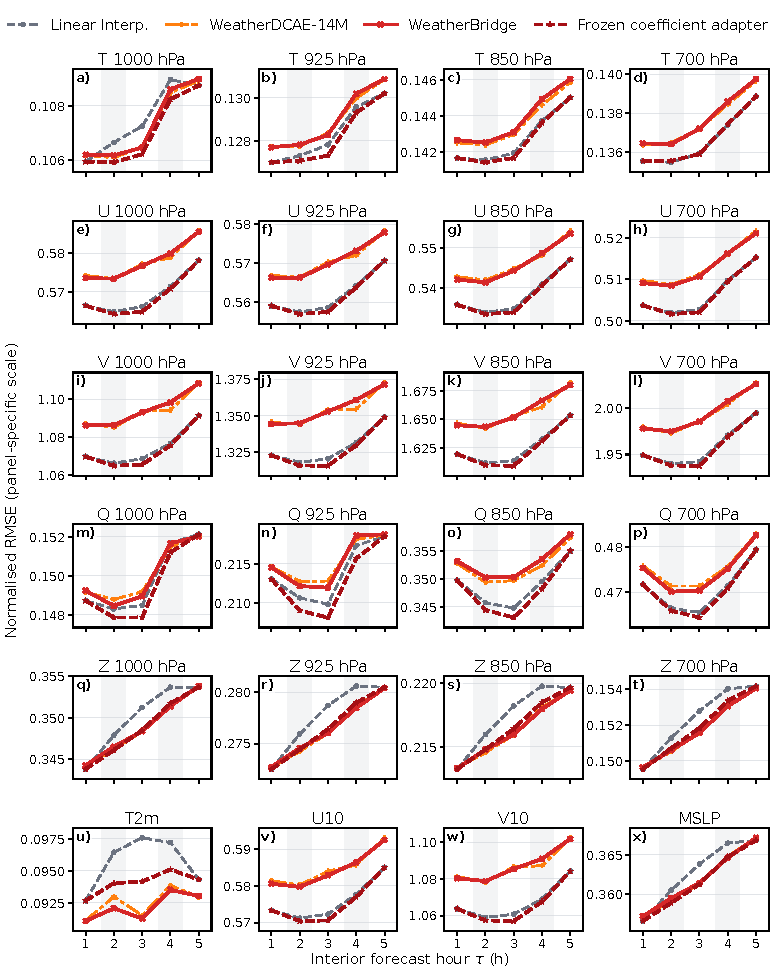
\includegraphics[width=\textwidth,height=0.84\textheight,keepaspectratio]{images/fig_nwp_adapter_2022_6h.pdf}
\caption{IFS HRES anchor interpolation against ERA5 for 16 independent 2022
initialisations. The 24 panels follow the five hours inside a six-hour anchor
interval; $\tau$ is interior offset, not forecast lead. Curves show Linear
Interp., WeatherDCAE-14M, raw WeatherBridge and the frozen coefficient
adapter. Grey bands mark the held-out hours $\tau\in\{2,4\}$; ranges are
panel-specific. Only the adapter-versus-Linear comparison is confirmatory.
The endpoint guard ties $\tau\in\{1,5\}$ exactly; T700 at $\tau=2$ and 4
contains the only regressions.}
\label{fig:nwp_adapter_2022}
\end{figure}

\FloatBarrier
\newgeometry{margin=18mm}
\begin{supplementlandscape}
\noindent
\begin{minipage}{\linewidth}
\setstretch{1}
\setlength{\abovecaptionskip}{3pt}
\section{Reference architecture schematics}

Supplementary Fig.~\ref{fig:reference_architectures} summarises the
comparator architectures defined in Methods.

\centering
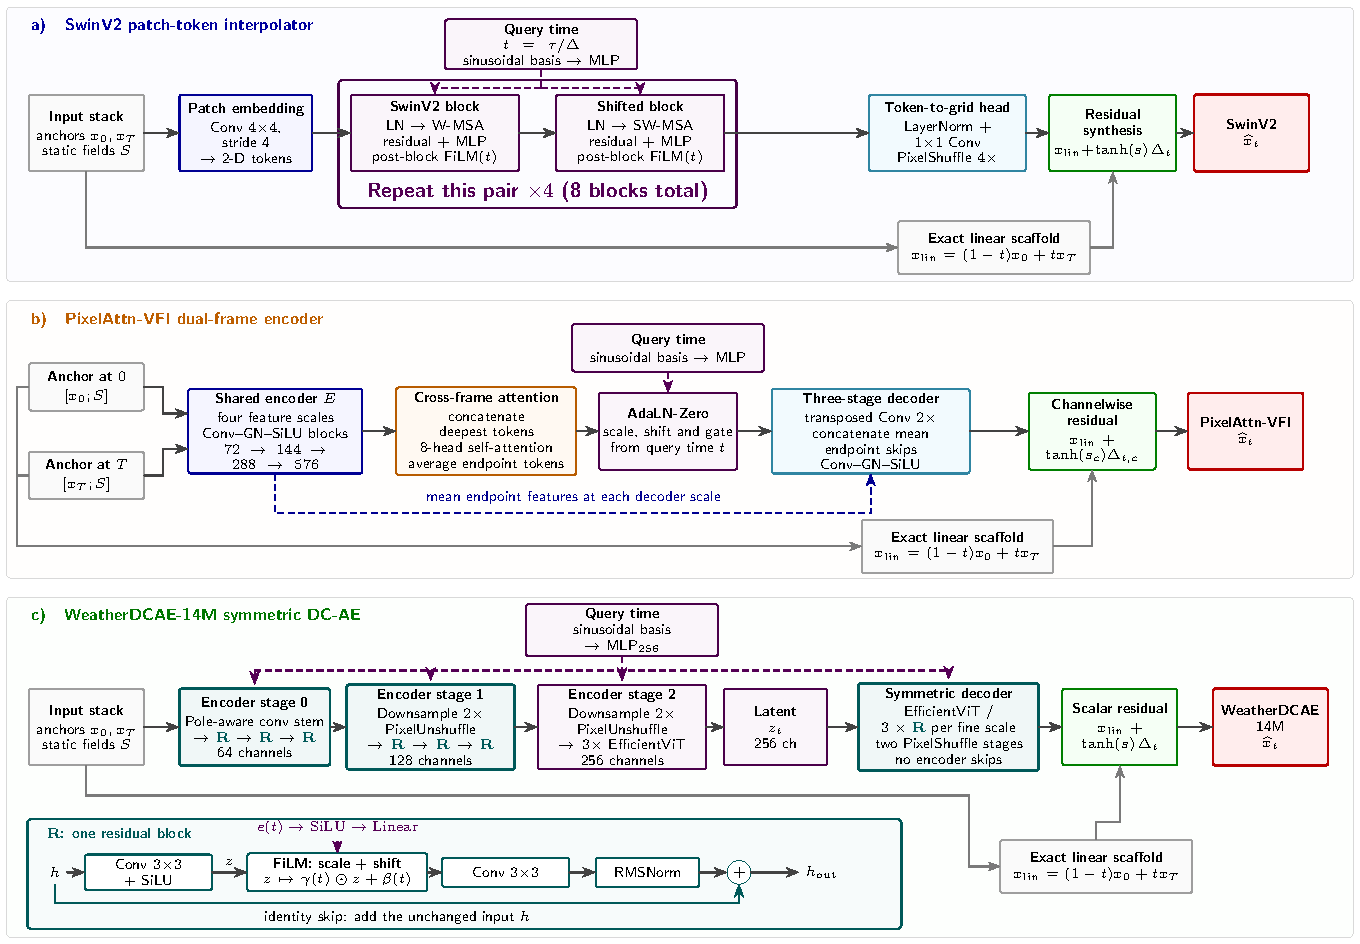
\includegraphics[width=0.98\linewidth,height=0.74\textheight,keepaspectratio]{images/fig_reference_architectures.pdf}
\captionof{figure}{Reference architectures used in the principal comparison.
\textbf{a)} SwinV2 alternates windowed and shifted-window attention on patch
tokens, with time-conditioned FiLM after each block.
\textbf{b)} PixelAttn-VFI shares the endpoint encoder, mixes deepest tokens
through attention, and conditions the bottleneck on time. Mean endpoint
features supply decoder skips.
\textbf{c)} WeatherDCAE-14M has no cross-scale encoder--decoder skips.
Read stages top to bottom: Conv--PixelUnshuffle halves height and width,
then three blocks run sequentially. Channel counts denote feature width.
Teal $R$ blocks occur at 64 and 128 channels in both encoder and decoder;
the deepest stage uses EfficientViT multiscale linear attention.
The inset expands one $R$: Conv--SiLU, FiLM, Conv and RMSNorm act sequentially,
then add the unchanged input $h$ through the identity skip. FiLM applies
channelwise scale and shift derived from time embedding $e(t)$.
Convolutions in $R$ use pole-aware boundaries. Purple dashed arrows carry
time conditioning; blue carries endpoint skips. Each model adds a scaled
correction to linear interpolation.}
\label{fig:reference_architectures}
\end{minipage}
\end{supplementlandscape}
\restoregeometry

\FloatBarrier
\section{S-DYff ensemble averaging}
\label{sec:sdyff-ensemble}

S-DYff-ENS averages 21 stochastic reconstructions from the S-DYff checkpoint.
The plotted S-DYff curve retains the original single reconstruction used in
the tables. For a paired estimate of the averaging effect, we also recomputed
$N=1,4,16,21$ using nested prefixes of the same random draws. Relative to
this paired $N=1$ control, $N=21$ reduces aggregate normalised RMSE by
0.69--0.89\% across the six year--interval combinations and by
0.67--0.87\% at held-out hours. The paired control is a new draw, so these
percentages need not equal the difference from the archived S-DYff curve.
Seven-day block-bootstrap intervals describe variation across evaluation
dates conditional on the sampling seed, not variation across sampling seeds.

All 24 fields are shown for full-year 2020 and 2021 and the fixed 48-anchor
2022 sample. The six-hour 2020, twelve-hour 2020 and six-hour 2021 panels
appear earlier in the main text and Supplementary Information; the remaining
three comparisons appear in Supplementary Figs.~\ref{fig:supp_ens_12h_2021},
\ref{fig:supp_ens_6h_2022} and \ref{fig:supp_ens_12h_2022}.
Ensemble results cover RMSE and ACC only. The
spectral, HRES and full-query supervision experiments retain their original
inference settings.

\begin{figure}[p]
\centering
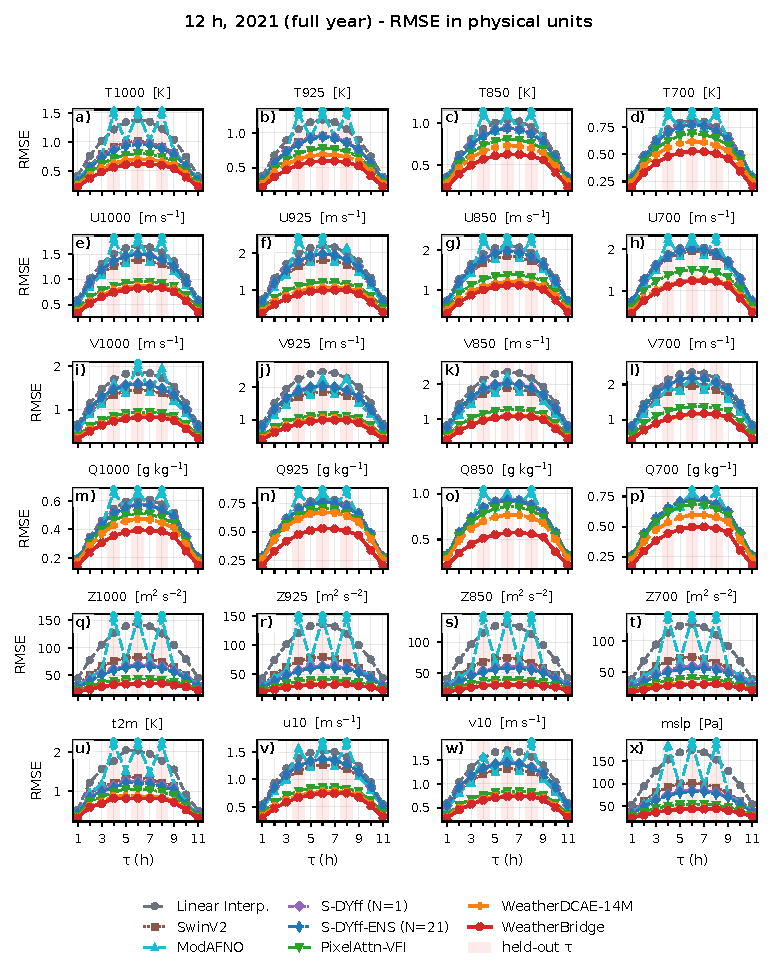
\includegraphics[width=\textwidth,height=0.80\textheight,keepaspectratio]{images/fig_channels_all_12h_2021_phys.pdf}
\caption{Twelve-hour physical-unit RMSE for all 24 fields over full-year 2021.
S-DYff ($N=1$) and S-DYff-ENS ($N=21$) use the same checkpoint. Shading marks
held-out query hours; upward arrows mark clipped ModAFNO values.}
\label{fig:supp_ens_12h_2021}
\end{figure}

\begin{figure}[p]
\centering
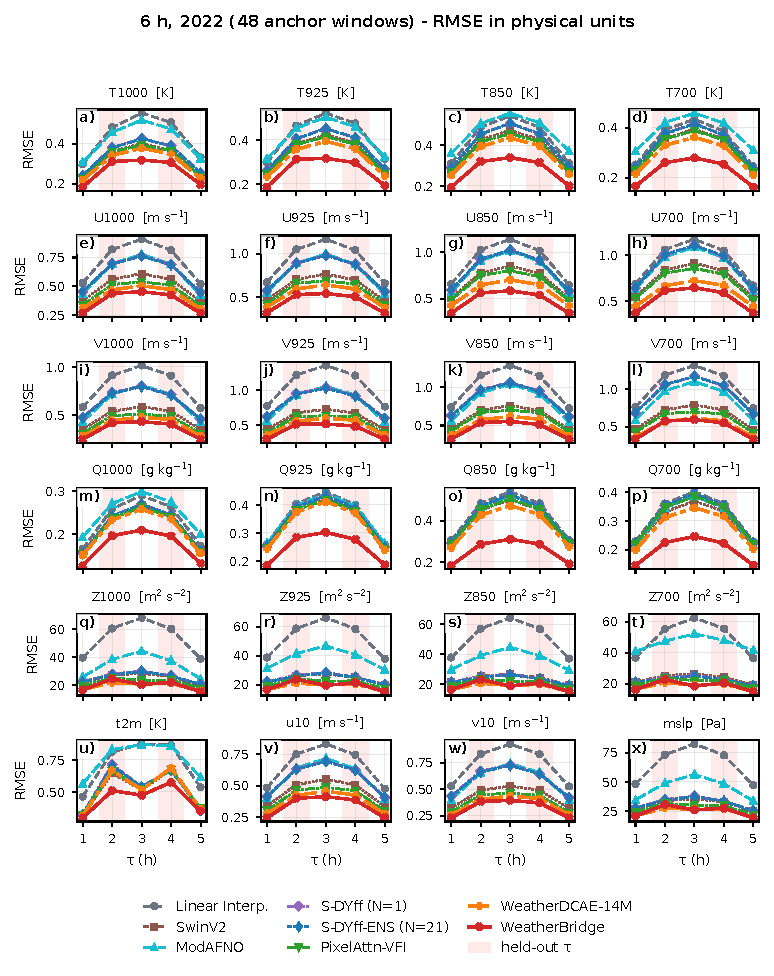
\includegraphics[width=\textwidth,height=0.80\textheight,keepaspectratio]{images/fig_channels_all_6h_2022_phys.pdf}
\caption{Six-hour physical-unit RMSE for all 24 fields on the fixed
48-anchor 2022 sample. S-DYff ($N=1$) is the archived single reconstruction;
S-DYff-ENS ($N=21$) averages outputs from the same checkpoint. Shading marks
held-out query hours.}
\label{fig:supp_ens_6h_2022}
\end{figure}

\begin{figure}[p]
\centering
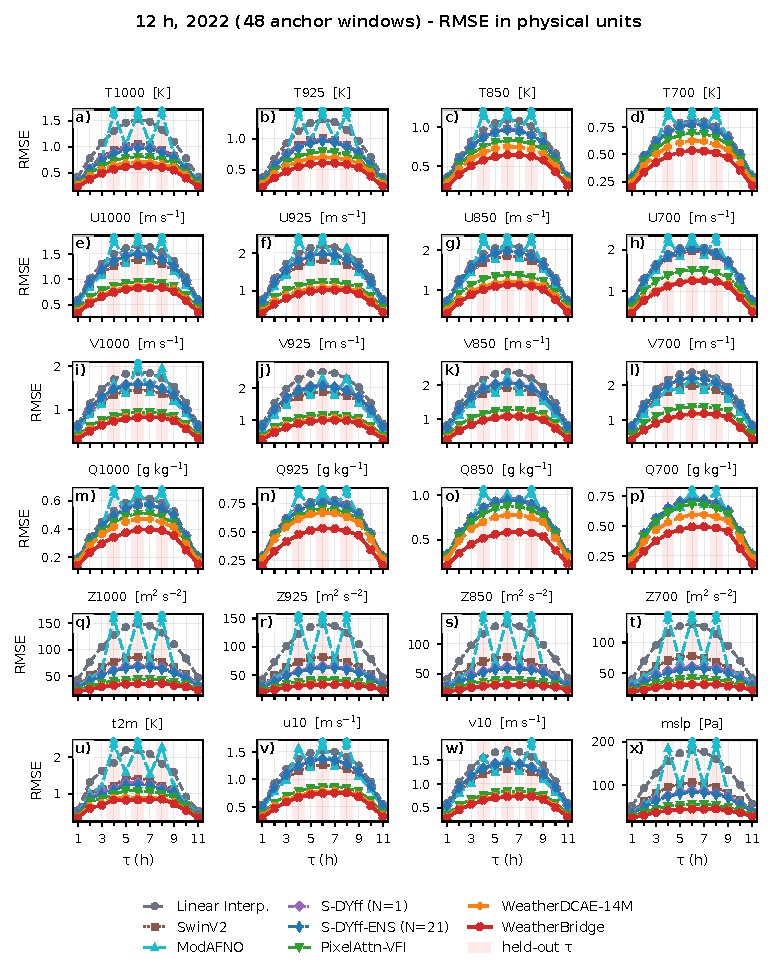
\includegraphics[width=\textwidth,height=0.80\textheight,keepaspectratio]{images/fig_channels_all_12h_2022_phys.pdf}
\caption{Twelve-hour physical-unit RMSE for all 24 fields on the fixed
48-anchor 2022 sample. Model labels follow Supplementary
Fig.~\ref{fig:supp_ens_6h_2022}. Shading marks held-out query hours; upward
arrows mark clipped ModAFNO values.}
\label{fig:supp_ens_12h_2022}
\end{figure}

\FloatBarrier
\end{document}
